\chapter{User Guide}
	\section{Guide for game users}
	This guide is aimed at users that might have to switch on the game and follow basic steps to play it. It does not incorporate any admin knowledge and switching on the other parts of the game. That will be outlined in the next chapter.

	To start the game you will need to find the package and run it. This is done by simply switching on the GuiUser package from terminal using the jar command for Java. If you see the following message: 

	\begin{figure}[htp]
		\centering
		\makebox{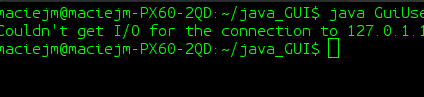
\includegraphics[width=0.4\hsize]{figures/IOError.png}}
		\caption{Input Output error from the server.}
	\end{figure}

	It means that the server is down and you need to contact the application administrator to get it up before you can run the game. If that has happened you will be presented with the following screen:

	\begin{figure}[htp]
		\centering
		\makebox{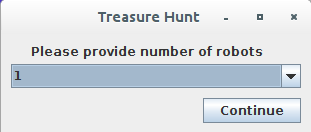
\includegraphics[width=0.4\hsize]{figures/App1.png}}
		\caption{Number of robots prompt.}
	\end{figure}

	This means that the application is ready to start playing the game. If you select the number of robots you should then be presented with the following screen:

	\begin{figure}[htp]
		\centering
		\makebox{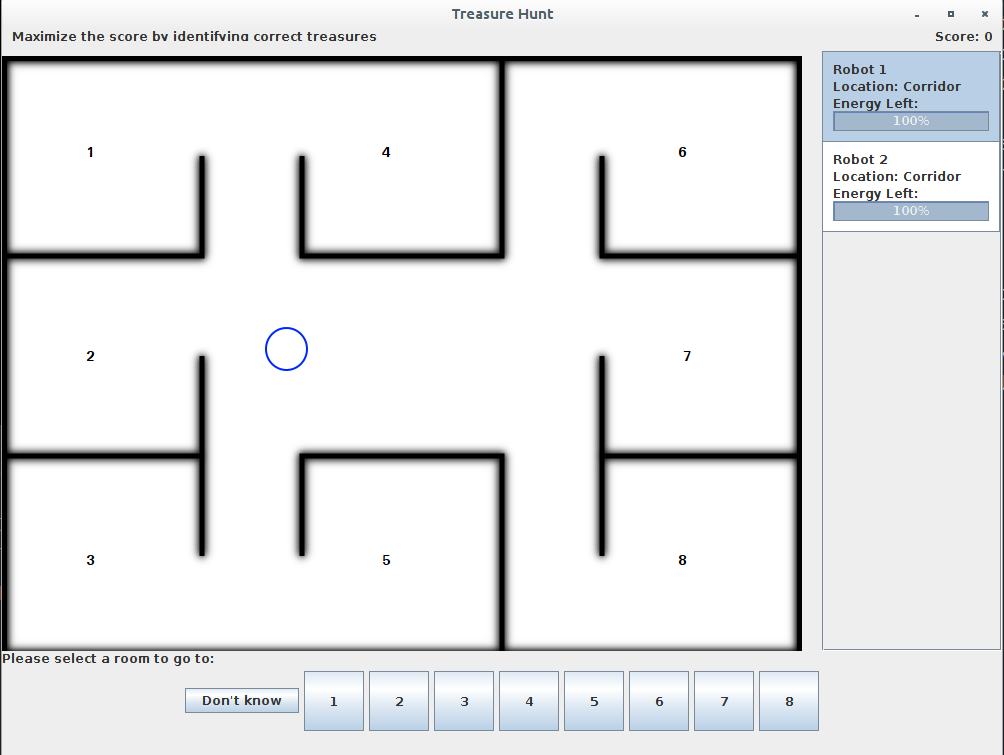
\includegraphics[width=0.4\hsize]{figures/finished.png}}
		\caption{Full GUI.}
	\end{figure}

	This is the UI interface from which you can play the game. Once you select a room a robot will engage in a conversation with you whether or not you wish to visit the room: \\
	\begin{figure}[htp]
		\centering
		\makebox{
\includegraphics[width=0.4\hsize]{figures/App2.png}}
		\caption{Dialogue prompt}
	\end{figure}
	If so, the robot will set itself to a traveling state until it reaches that room. \\
	\begin{figure}[htp]
		\centering
		\makebox{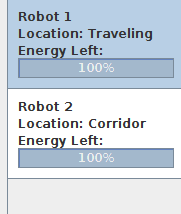
\includegraphics[width=0.4\hsize]{figures/App3.png}}
		\caption{Robot traveling.}
	\end{figure}
	You can also select another robot if you selected more than one robot to control at the start. If that's so please notice that the room that you sent your previous robot to will not be click-able. This just means you can choose each room once so choose wisely.
	\begin{figure}[htp]
		\centering
		\makebox{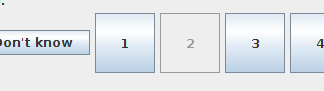
\includegraphics[width=0.4\hsize]{figures/App4.png}}
		\caption{Room no longer click-able.}
	\end{figure}
	Once the robot arrives to its destination. You will be prompted about the treasure footprint and colour that the robot discovered. You will be able to choose a treasure from a set of desired ones. These treasures will closely identify to the colour or footprint so you can make the decision now or take a picture.
	\begin{figure}[htp]
		\centering
		\makebox{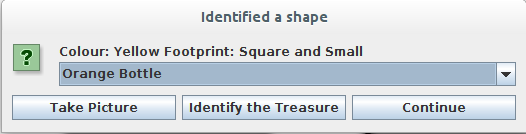
\includegraphics[width=0.3\hsize]{figures/App5.png}}
		\caption{Prompt regarding robot finding the treasure.}
	\end{figure}

	Before clicking identify the treasure you should always make sure that you select a treasure from the drop-down list first otherwise the first selection on that list will be carried out which would not be ideal. Remember that taking pictures costs so try to minimize the need to do so. For now take a picture for learning purposes.

	\begin{figure}[htp]
		\centering
		\makebox{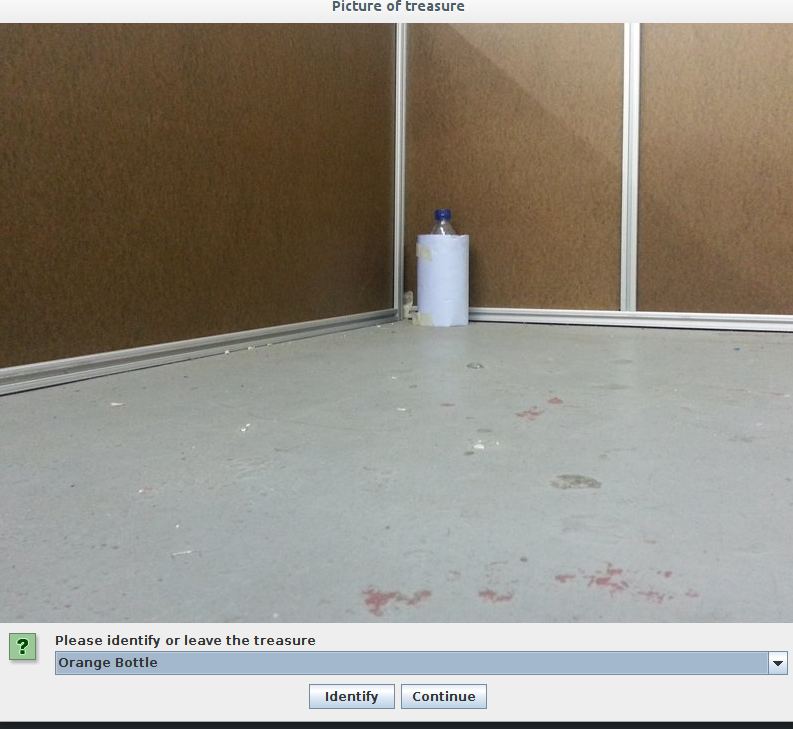
\includegraphics[width=0.3\hsize]{figures/App6.png}}
		\caption{Effect of taking a picture}
	\end{figure}

	You are now presented with a picture of the treasure and should be able to deduce what you are seeing but you can still press continue to forfeit the treasure. If you however identify and treasure you will receive a reply similar to this one:

	\begin{figure}[htp]
		\centering
		\makebox{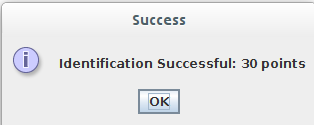
\includegraphics[width=0.3\hsize]{figures/App7.png}}
		\caption{Effect of taking a picture}
	\end{figure}

	Continue the previous steps and try to maximize the score as well as visit all the rooms. When you either visit all the rooms or the energy runs out from your robots you will finish the game. At that point you will receive the following type of message:
	\begin{figure}[htp]
		\centering
		\makebox{
\includegraphics[width=0.4\hsize]{figures/App8.png}}
		\caption{Effect of taking a picture}
	\end{figure}